\documentclass{llncs}
\usepackage{graphicx}
\usepackage{url}
\usepackage[utf8]{inputenc} % Umlaute


\begin{document}

\title{Evaluation of a Visualization Component for the Differencegraph}
\author{Firstname Lastname\inst{1} \and Firstname Lastname\inst{2}}
\institute{Universität Wien \\ Währinger Straße 29 \\ 1090 Wien}
\maketitle
\begin{abstract}
...
\end{abstract}

\section{Introduction}
\label{sec:Introduction}

Research question: Which visualization should be used for the Differencegraph?





\section{Differencegraph Model and Visualization}
\label{sec:DiffgraphModel}
The differencegraph concept \cite{lit:VisuApprDiffAnalysis} consists of two parts one is the model and the other is the visualization of this model.

Explain model and calculation, explain different markings (5)

Don't explain 3 markings. 




The idea behind the visualization of the difference model is to represent each of the markings with different styles. For example each marking can be mapped to represent a specific symbol. This symbol can then be visualized on nodes and edges. To ensure an appropriate visualization is taken a survey was conducted.



\section{Evaluation}
\label{sec:Evaluation}
To address the research question, stated in Section 1, an online survey was conducted. An online survey is well suited for this kind of research it offers a 

Based on a literature research nine different styles for visualizing the difference graph where extracted. From these nine styles the best one should be found with this evaluation.



\subsection{Design}
\label{sec:Design}

\subsection{Procedure}
\label{sec:Procedure}
After finalizing the surveys design a two-sided pretest was conducted. In the first pretest a discussion with two people took place where the overall question and answer wording was adapted to support the users understanding. In our second pretest five people had to complete the survey and give advices what should be changed. 

After the pretest the survey was executed with 73 participants from which 31 completed the survey.

\subsection{Results}
\label{sec:Results}



\begin{figure}
	\centering
	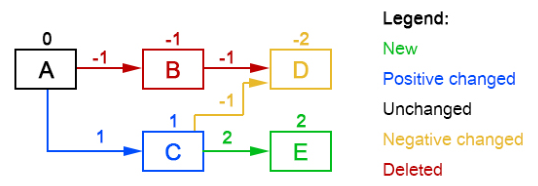
\includegraphics[width=0.8\textwidth]{Images/ColorCodedGraph.PNG}
	\caption{Final Representation of the Differencegraph}
	\label{fig:DiffGraphVisualization}
\end{figure}

\section{Applications}
\label{sec:Applications}

Merging of processes -> Before merging two processes seeing where they differ from each other can be really good and support the merge process. For example activities which are only executed in one of the processes can be obtained easily.

Comparing two instances -> For example two factories which produce by same input the same output. Are there differences in process execution?

Evolution of a process -> Compare year 2013 and 2014, what has changed?


\section{Related Work}
\label{sec:RelatedWork}

Difference between the differencegraph concept and conformance checking?

\section{Conclusion}
\label{sec:Conclusion}


\bibliography{Literature}
\bibliographystyle{plain}

\end{document}
